\documentclass{beamer}

\usepackage{lmodern}
\usepackage[french]{babel}
\usepackage[utf8]{inputenc}
\usepackage[T1]{fontenc}

\usetheme{Warsaw}
\setbeamerfont{page number in head/foot}{size=\large}
\setbeamertemplate{footline}[frame number]
\beamertemplatenavigationsymbolsempty
\date{}
\author{Arthur Burgada \and Pierre-Huges Blelly}

\title{Détection des ondes gravitationnelles}
\begin{document}

\begin{frame}
	\titlepage
\end{frame}

\begin{frame}
	\frametitle{Plan de l'exposé}
	\tableofcontents
\end{frame}

\section{Les ondes gravitationnelles}
\begin{frame}
	\frametitle{Découverte théorique}
	\begin{itemize}
		\item 1916 : Relativité Générale de Einstein
		\item En linéarisant les équations un terme d'onde progressive apparaît
		\item Artefact mathématique ou réalité physique ?
	\end{itemize}
\end{frame}

\begin{frame}
	\begin{itemize}
		\item Analogue à onde électromagnétique : émis lorsque un corps massique accélère
		\item Vitesse de propagation c
		\item Mais décroissance en 1/R
		\item Amplitude extrêmement faible
		\bigskip
		\center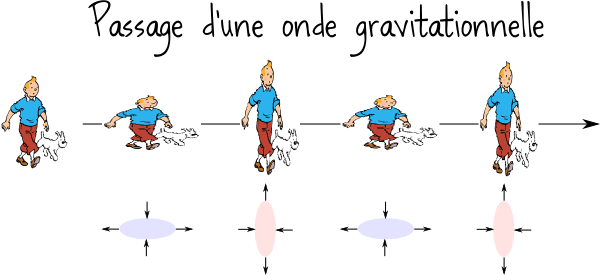
\includegraphics[scale = 0.4]{Docs/tintin.png}
	\end{itemize}

\end{frame}


\begin{frame}
	\frametitle{Mise en évidence indirecte : Pulsar de Hulse et Taylor}
	\begin{columns}
	\begin{column}{0.5\textwidth}
		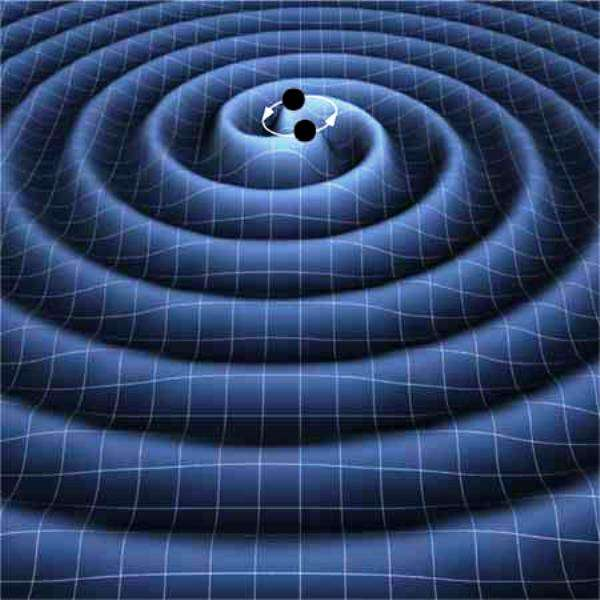
\includegraphics[scale=0.2]{Docs/pulsar_binaire.jpeg}
	\end{column}
	\begin{column}{0.5\textwidth}
	\begin{itemize}
		\item Couple de 2 étoiles dont l'une est une étoile à neutrons
		\item PSR B1913+16 découvert en 1974
	\end{itemize}
	\end{column}
	\end{columns}
\end{frame}

\begin{frame}
	\frametitle{Mise en évidence indirecte : Pulsar de Hulse et Taylor}
	\begin{columns}
	\begin{column}{0.5\textwidth}
		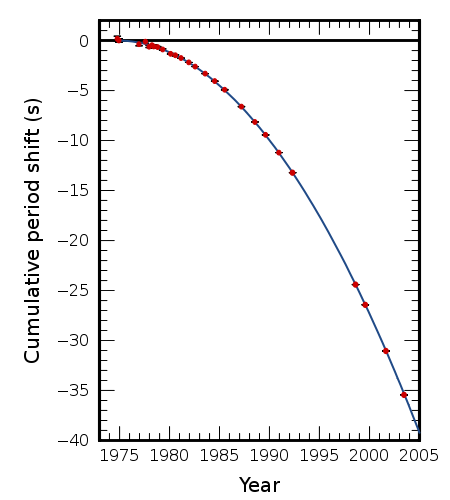
\includegraphics[scale=0.3]{Docs/period_shift_pulsar.png}
	\end{column}
	\begin{column}{0.5\textwidth}
		\begin{itemize}
			\item Période de 7,75 heures
			\item Diminution de la période dûe à l'émission d'ondes gravitationnelles
		\end{itemize}

	\end{column}
	\end{columns}
\end{frame}

\begin{frame}
	\frametitle{Enjeux du projet LIGO/VIRGO}
	\begin{itemize}
		\item Mise en évidence directe
		\item Précision suffisante
		\item Evaluer le taux d'expansion de l'Univers de manière indépendante de la technique utilisant la luminosité des supernovas
	\end{itemize}

\end{frame}


\section{Présentation du Michelson}

\begin{frame}
	\frametitle{Interféromètre de Michelson}
	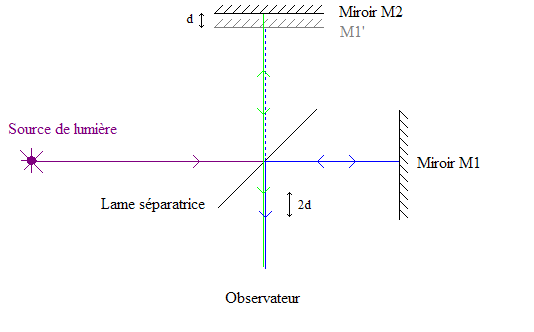
\includegraphics[scale=0.5]{Docs/interferometre_michelson.png}
\end{frame}


\section{Présentation des interféromètres LIGO / VIRGO}
\begin{frame}
	\frametitle{L'interféromètre VIRGO}
	\begin{columns}
		\begin{column}{0.5\textwidth}
			\small
			\begin{enumerate}[-]
				\item 2 bras de 4km de long parfaitement horizontaux (Sous Vide)
				\item Système complètement isolé de l'exterieur
			\end{enumerate}
		\end{column}
		\begin{column}{0.5\textwidth}
			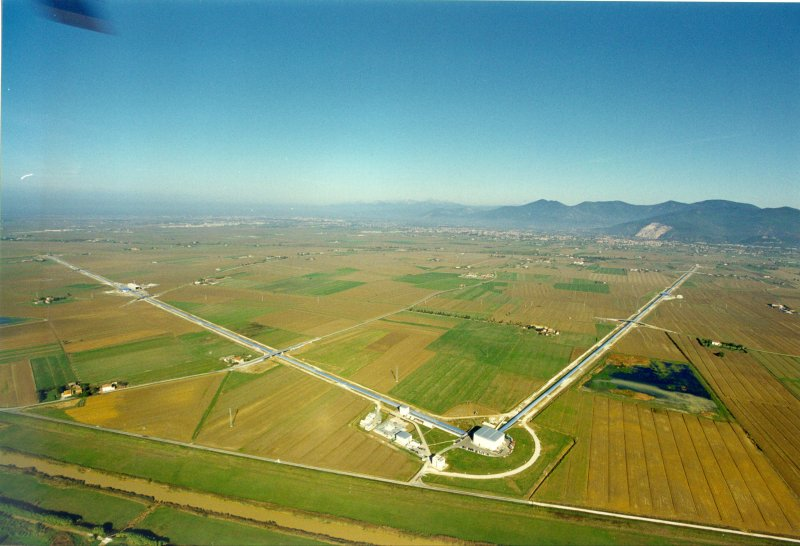
\includegraphics[scale=.5]{Docs/virgoview.png}
		\end{column}
	\end{columns}
	\bigskip
	2 interféromètres: VIRGO (Italie) et LIGO(Hanford(Washington) / Livinston (Louisianne))
\end{frame}
\section{LASER}


\begin{frame}
	\frametitle{Système injection}
	2 Lasers: Un laser maître et un laser esclave
	\break

	On injecte un rayonnement laser dans la cavité du second laser pour faire change son gain et modifier la fréquence d'émission du second laser.
\end{frame}

\begin{frame}
	\frametitle{Le laser de LIGO}
	Fonctionne en quatre étapes
	\begin{enumerate}[1.]
		\item Emission du laser Maître par une photodiode
		\item Emission du laser Esclave
		\item Première amplification
		\item Seconde amplification 
	\end{enumerate}
\end{frame}
\end{document}
